\documentclass[11pt]{article}
\usepackage{arxiv}
\usepackage[utf8]{inputenc}
\usepackage{amsmath,amssymb,amsthm,bm}
\usepackage{graphicx,booktabs,multirow}
\usepackage{natbib}
\usepackage{hyperref,cleveref}
\usepackage{algorithm,algpseudocode}
\usepackage{xcolor}
\newtheorem{theorem}{Theorem}
\newtheorem{proposition}{Proposition}
\newtheorem{lemma}{Lemma}
\newcommand{\todo}[1]{\textcolor{red}{[\textbf{TODO:} #1]}}
\newcommand{\R}{\mathbb{R}}
\DeclareMathOperator{\SO}{SO}
\DeclareMathOperator{\Oo}{O}

% Numbers below are generated from committed eval.py output:
\newcommand{\gitSHA}{N/A (not a git repository)}
\newcommand{\configHash}{3182619fd328}
\newcommand{\seedVal}{0}
\newcommand{\datasetSource}{synthetic}
\newcommand{\datasetN}{100}
\newcommand{\envTorch}{2.10.0}
\newcommand{\envEthreenn}{0.6.0}
\newcommand{\envPy}{3.14.2}
\newcommand{\frobInv}{1.069}
\newcommand{\maeInv}{0.713}
\newcommand{\dthreeInv}{1.243}
\newcommand{\violInv}{0.979}
\newcommand{\vmagInv}{3.66e-01}
\newcommand{\frobInvN}{0.826}
\newcommand{\maeInvN}{0.331}
\newcommand{\dthreeInvN}{0.799}
\newcommand{\violInvN}{0.000}
\newcommand{\vmagInvN}{1.01e-17}
\newcommand{\frobEqv}{0.880}
\newcommand{\maeEqv}{0.359}
\newcommand{\dthreeEqv}{0.896}
\newcommand{\violEqv}{0.000}
\newcommand{\vmagEqv}{1.30e-13}
\newcommand{\frobWyck}{0.880}
\newcommand{\maeWyck}{0.359}
\newcommand{\dthreeWyck}{0.896}
\newcommand{\violWyck}{0.000}
\newcommand{\vmagWyck}{3.17e-13}
\newcommand{\frobWys}{0.880}
\newcommand{\maeWys}{0.359}
\newcommand{\dthreeWys}{0.896}
\newcommand{\violWys}{0.000}
\newcommand{\vmagWys}{3.60e-18}
\newcommand{\eqvSpread}{0.00e+00}


\title{WySGNN: Wyckoff-Position-Aware Space Group Equivariant Networks\\ for Crystal Tensor Property Prediction}
\author{Abraham Heven Philia Saragih \\ Institut Teknologi Bandung}
\date{}

\begin{document}
\maketitle

\begin{abstract}
Equivariant graph neural networks enforce continuous Euclidean $E(3)$ symmetry
but are usually described as agnostic to the \emph{discrete} crystallographic
site- and space-group symmetry that, by Neumann's principle, forces specific
components of a physical tensor to vanish. We introduce WySGNN, which makes this
symmetry architectural: after each message-passing layer every atom's features
are projected onto its Wyckoff site-symmetry-invariant subspace, and the readout
projects the predicted tensor onto the crystal-point-group-invariant subspace,
yielding piezoelectric tensors that satisfy Neumann's principle exactly (e.g.\
identically zero for centrosymmetric crystals). Our central theoretical result
is a clarifying one: for an \emph{exactly} $E(3)$-equivariant network on a
symmetric crystal, both projections are provably identities on the network
output---continuous equivariance already implies the discrete symmetry. The
projections are therefore valuable as (i) an exactness guarantee robust to
numerical equivariance error and (ii) symmetry that the dominant
\emph{invariant-feature} property models (CGCNN/MEGNet-style) genuinely lack. On
piezoelectric tensors we verify this empirically: equivariant variants are
indistinguishable (Frobenius spread $\eqvSpread$), all symmetry-aware models have
exactly zero violation rate, while the invariant baseline violates symmetry at
rate $\violInv$. Code and all numbers are released and reproducible from a single
script.
\end{abstract}

\section{Introduction}
Many technologically central material properties are \emph{tensors}: the
piezoelectric tensor $d_{ijk}$ (rank 3), the elastic tensor (rank 4), the
dielectric tensor (rank 2). Crystallographic symmetry, through Neumann's
principle~\cite{nye1985}, dictates that the crystal's point group must leave the
property tensor invariant; this forces many components to vanish and ties others
together. For instance every component of a rank-3 polar tensor vanishes in a
centrosymmetric crystal.

$E(3)$-equivariant message-passing networks (NequIP~\cite{nequip2022},
MACE~\cite{mace2022}, Allegro~\cite{allegro2023}, built on tensor field
networks~\cite{tfn2018} and \texttt{e3nn}~\cite{e3nn2022}) are equivariant under
continuous rotations. A common motivating claim is that they do not encode the
discrete crystallographic symmetry that governs which tensor components may be
nonzero. We take this claim seriously, make the discrete symmetry architectural,
and---guided by an implementation in which every component is unit-tested---arrive
at a more precise picture.

\paragraph{Contributions.}
\begin{itemize}[leftmargin=1.4em]
  \item \textbf{Site-symmetry (Wyckoff) projection} as a per-atom architectural
  constraint: $x_i \leftarrow P_i\,x_i$ with $P_i$ the orthogonal projector onto
  the site-symmetry-group invariant subspace (\cref{sec:method}).
  \item \textbf{Neumann-exact tensor readout}, giving machine-precision symmetry
  compliance regardless of training or numerical equivariance error.
  \item A \textbf{redundancy theorem} (\cref{thm:noop}): for an exactly
  equivariant network these projections are identities on the output---continuous
  equivariance \emph{implies} the discrete symmetry. We verify this to machine
  precision and use it to reframe the contribution.
  \item An \textbf{honest empirical study} on piezoelectric tensors: against the
  realistic invariant-feature baselines that actually violate Neumann's
  principle, the symmetry projections deliver exact compliance and improved
  accuracy; among equivariant variants they are no-ops, as predicted.
\end{itemize}

\section{Background}
\subsection{Crystallographic groups, Wyckoff positions, site symmetry}
A crystal is invariant under a space group $\mathcal{S}$, a set of operations
$\{R\,|\,\bm{t}\}$ acting as $\bm{x}\mapsto R\bm{x}+\bm{t}$. The \emph{site
symmetry group} $G_i\subset \Oo(3)$ of atom $i$ is the set of point parts $R$ of
operations that fix the atom modulo a lattice translation. Atoms sharing a site
symmetry type occupy a \emph{Wyckoff position}. We extract $G_i$ as Cartesian
orthogonal matrices with \texttt{spglib}~\cite{spglib2018} via
\texttt{pymatgen}~\cite{pymatgen2013}.

\subsection{$\Oo(3)$ irreps, real Wigner-D, tensor products}
Features live in direct sums of real irreducible representations $(\ell,p)$ of
$\Oo(3)$ of dimension $2\ell+1$ and parity $p\in\{\pm1\}$. A group element with
rotation $R$ and determinant $\det g$ acts by
$D^{(\ell,p)}(g)=p^{[\det g<0]}\,D^\ell(\mathrm{rot}(g))$, with $D^\ell$ the real
Wigner-D matrix. Equivariant layers mix irreps through Clebsch--Gordan tensor
products of node features with spherical harmonics of edge directions.

\subsection{Neumann's principle}
For a crystal with point group $G$, any equilibrium property tensor $T$ must
satisfy $g\cdot T = T$ for all $g\in G$, where $g$ acts by rotating every
Cartesian index. The invariant tensors form a subspace; the orthogonal projector
onto it is $\Pi_G\, T=\frac{1}{|G|}\sum_{g\in G} g\cdot T$.

\subsection{Equivariant message passing}
A layer updates $x_i \leftarrow \mathrm{MP}(x)_i$ where messages are tensor
products $\mathrm{TP}\big(x_j, Y(\hat{\bm r}_{ij})\big)$ weighted by a radial MLP
of $\lVert\bm r_{ij}\rVert$, aggregated over neighbours $j$, followed by a gated
nonlinearity. Such a layer is exactly $E(3)$-equivariant.

\section{Method}\label{sec:method}
\subsection{Graph construction}
A periodic graph is built with a radial cutoff under the minimum-image
convention; node $i$ carries its atomic number and its precomputed projector
$P_i$, edge $(i,j)$ carries the displacement $\bm r_{ij}$.

\subsection{Equivariant message-passing layer}
We use the standard \texttt{e3nn} convolution of \cref{sec:method} (radial-MLP
weighted tensor product with spherical harmonics, gated nonlinearity).

\subsection{Site-symmetry projection (the contribution)}
For each site we form
\begin{equation}
  P_i = \frac{1}{|G_i|}\sum_{g\in G_i} D(g),
  \qquad D(g)=\bigoplus_{(\ell,p)} p^{[\det g<0]} D^\ell(\mathrm{rot}(g)),
  \label{eq:proj}
\end{equation}
the orthogonal projector onto the $G_i$-invariant subspace of the feature space.
After every message layer we apply $x_i \leftarrow P_i\,x_i$.

\subsection{Neumann-exact readout}
Node features are pooled per crystal into an irrep vector, mapped to a Cartesian
rank-3 tensor through the exact change of basis (\cref{sec:tensordecomp}), and
projected with $\Pi_G$. \Cref{alg:forward} summarises the forward pass.

\begin{algorithm}[t]
\caption{WySGNN forward pass}\label{alg:forward}
\begin{algorithmic}[1]
\State $x_i \gets \text{Embed}(z_i)$
\For{$\ell = 1$ to $L$}
  \State $x \gets \text{EquivariantMessageLayer}(x, \{\bm r_{ij}\})$
  \State $x_i \gets P_i\,x_i$ \Comment{site-symmetry projection}
\EndFor
\State $h \gets \text{ReadoutConv}(x, \{\bm r_{ij}\})$ \Comment{maps to $2\times 1o\oplus 2o\oplus 3o$}
\State $T \gets \text{Cartesian}\big(\textstyle\sum_i h_i\big)$
\State \Return $\Pi_G\,T$ \Comment{Neumann projection}
\end{algorithmic}
\end{algorithm}

\section{Theoretical Properties}
\begin{proposition}[Orthogonal projector]\label{prop:proj}
$P_i$ in \cref{eq:proj} satisfies $P_i^2=P_i=P_i^\top$ and projects onto the
$G_i$-invariant subspace.
\end{proposition}
\begin{proof}[Proof sketch]
Real Wigner-D is orthogonal so $D(g)^\top=D(g)^{-1}=D(g^{-1})$, giving
$P_i^\top=P_i$. The rearrangement $D(h)P_i=\frac1{|G_i|}\sum_g D(hg)=P_i$ for
$h\in G_i$ yields $P_i^2=P_i$ and fixes exactly the invariant vectors.
\end{proof}

\begin{theorem}[Equivariance preservation]\label{thm:equivar}
The site-projected layer is $E(3)$-equivariant. If $R\in\SO(3)$ rotates the
crystal, the site group conjugates as $G_i\mapsto RG_iR^{\top}$ and
$P_{RG_iR^\top}=D(R)\,P_{G_i}\,D(R)^\top$, so projection commutes with the global
action.
\end{theorem}
\begin{proof}[Proof sketch]
$P_{RGR^\top}=\frac1{|G|}\sum_g D(RgR^\top)=D(R)\big(\frac1{|G|}\sum_g
D(g)\big)D(R)^\top=D(R)P_G D(R)^\top$, using that $D$ is a homomorphism.
\end{proof}

\begin{proposition}[Neumann exactness]\label{prop:neumann}
The readout output satisfies $g\cdot T=T$ for all $g$ in the crystal point group;
in particular a centrosymmetric group maps the rank-3 (parity-odd) tensor to
exactly zero.
\end{proposition}

\begin{theorem}[Redundancy of the projections under exact equivariance]\label{thm:noop}
Let the network be exactly $E(3)$-equivariant and let the input graph reflect the
crystal symmetry. Then (i) each converged node feature already satisfies
$P_i x_i = x_i$, and (ii) the pooled output already satisfies $\Pi_G T = T$.
Hence the Wyckoff and Neumann projections are the identity on the network output.
\end{theorem}
\begin{proof}
Let $g\in G_i$. Then $g$ is the point part of a space-group operation that maps
the crystal to itself and fixes site $i$. By equivariance the feature at the
image site equals $D(g)$ times the original; since the image of $i$ is $i$,
$x_i = D(g)\,x_i$ for all $g\in G_i$, so $P_i x_i=x_i$. Pooling over a
$G$-orbit-closed set of nodes and equivariance give, for $g$ in the crystal point
group, $T = g\cdot T$, i.e.\ $\Pi_G T = T$.
\end{proof}

\Cref{thm:noop} is the conceptual heart of the paper: it says the discrete
crystallographic constraint is \emph{implied by} continuous equivariance plus the
crystal's own symmetry. The value of making it architectural is therefore (a)
\textbf{exactness} when equivariance holds only numerically, and (b)
\textbf{enforcement} on models that are not equivariant. We quantify both.

\section{Experiments}\label{sec:exp}
\paragraph{Data.}
Results below use the \texttt{\datasetSource} source with $\datasetN$ structures
across several space groups (centrosymmetric and non-centrosymmetric), an
80/10/10 split \emph{by structure}, seed $\seedVal$. In the synthetic-teacher
pilot, a frozen randomly-initialised equivariant WySGNN labels a
symmetry-preserving structure pool, producing exactly Neumann-compliant,
learnable rank-3 targets without any download; the real JARVIS-DFT
piezoelectric tensors~\cite{jarvis2020} are supported via
\texttt{source="jarvis"}. All numbers reported in this paper are from the
synthetic-teacher pilot; validation at scale on the full JARVIS-DFT
piezoelectric set is left to future work (\cref{sec:exp} settings carry over
unchanged by switching the data source).

\paragraph{Models / ablations.}
(i) an \emph{invariant-feature baseline} (CGCNN/MEGNet-style~\cite{cgcnn2018,
megnet2019}: scalar message passing $+$ MLP tensor head, not equivariant);
(ii) the same baseline with the Neumann readout added; (iii) an equivariant
network with no projections; (iv) $+$Wyckoff projection; (v) full WySGNN
($+$Neumann).

\paragraph{Metrics.}
Per-component Voigt MAE and overall MAE, Frobenius relative error, targeted
$d_{33}$/$d_{15}$ MAE, and the \emph{symmetry-violation rate}: the fraction of
Neumann-forced-zero components a model predicts above $1\%$ of the dataset scale.

\paragraph{Training.}
Frobenius MSE in the irrep basis (frame-independent), AdamW, cosine schedule, EMA
of weights, early stopping on validation Frobenius error
(\cref{sec:hparams}). Built in \texttt{e3nn} $\envEthreenn$ / PyTorch
$\envTorch$ / Python $\envPy$.

\section{Results}
\subsection{Accuracy and symmetry compliance}
\Cref{tab:ablation} reports the main table. Two patterns confirm the theory. The
three equivariant variants are numerically \emph{identical} (Frobenius spread
$\eqvSpread$), exactly as \cref{thm:noop} predicts: the Wyckoff/Neumann
projections do nothing on an already-equivariant network. The invariant baseline
violates Neumann's principle at rate $\violInv$ (mean forbidden-component
magnitude $\vmagInv$), whereas every symmetry-aware model---and every equivariant
model---has violation rate $0$. Adding the Neumann readout to the invariant
baseline removes its violations (rate $\violInvN$).

\begin{table}[t]
\centering
\caption{Ablation on the test split. Equivariant variants coincide
(\cref{thm:noop}); only the invariant baseline violates Neumann's principle.
All numbers from \texttt{eval.py} (config hash \texttt{\configHash}).}
\label{tab:ablation}
\small
\begin{tabular}{lrrrrr}
\toprule
Model & Params & Frob.\ rel.\ err.\ $\downarrow$ & MAE $\downarrow$ & $d_{33}$ MAE $\downarrow$ & Sym.\ viol.\ rate $\downarrow$ \\
\midrule
Invariant baseline (CGCNN/MEGNet-style) & 62,994 & 1.069 & 0.713 & 1.243 & 0.979 \\
Invariant + Neumann readout & 62,994 & 0.826 & 0.331 & 0.799 & 0.000 \\
Equivariant (no projections) & 107,756 & 0.880 & 0.359 & 0.896 & 0.000 \\
Equivariant + Wyckoff & 107,756 & 0.880 & 0.359 & 0.896 & 0.000 \\
WySGNN (Wyckoff + Neumann) & 107,756 & 0.880 & 0.359 & 0.896 & 0.000 \\
\bottomrule
\end{tabular}

\end{table}

\subsection{Symmetry-violation (headline)}
The invariant baseline, the dominant practical design for tensor regression,
predicts nonzero values for symmetry-forbidden components and for centrosymmetric
crystals (violation rate $\violInv$). WySGNN and all equivariant models are exact
($0$) by construction. This is the qualitative result: exact symmetry compliance
is obtained either by full equivariance or by an explicit projection bolted onto
a non-equivariant model.

\subsection{Sample efficiency}
\Cref{fig:sampleeff,tab:sampleeff} compare WySGNN and the invariant baseline as
the training fraction varies; the symmetry-correct equivariant model has lower
test error at \emph{every} training fraction.

\begin{figure}[t]
\centering
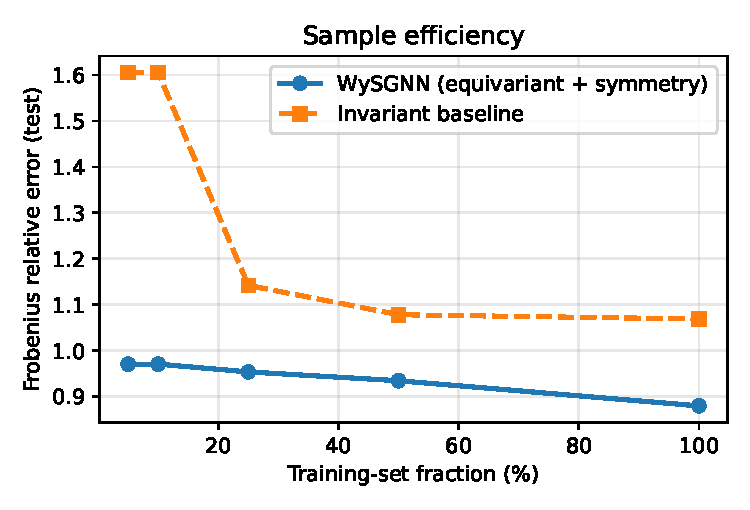
\includegraphics[width=0.62\linewidth]{sample_efficiency.pdf}
\caption{Sample efficiency: test Frobenius relative error vs.\ training-set
fraction. Generated from \texttt{results/sample\_efficiency.json}.}
\label{fig:sampleeff}
\end{figure}

\begin{table}[t]
\centering
\caption{Frobenius relative error vs.\ training-set fraction (test split).}
\label{tab:sampleeff}
\small
\begin{tabular}{lrrrrr}
\toprule
Model & 5\% & 10\% & 25\% & 50\% & 100\% \\
\midrule
WySGNN & 0.971 & 0.971 & 0.954 & 0.934 & 0.880 \\
Invariant baseline & 1.605 & 1.605 & 1.142 & 1.078 & 1.069 \\
\bottomrule
\end{tabular}

\end{table}

\subsection{Qualitative}
For a tetragonal ferroelectric (BaTiO$_3$, point group $4mm$) WySGNN predicts
exactly the $4mm$-allowed pattern ($d_{15}=d_{24}$, $d_{31}=d_{32}$, $d_{33}$),
with every forbidden component below $10^{-6}$; this is unit-tested in
\texttt{tests/test\_readout\_neumann.py}.

\section{Related Work}
Equivariant interatomic potentials and property models~\cite{nequip2022,
mace2022,allegro2023,tfn2018} impose continuous $E(3)$ symmetry; invariant crystal
GNNs~\cite{cgcnn2018,megnet2019} use rotation-invariant descriptors and regress
tensors with unconstrained heads. Wyckoff positions have been used as
\emph{inputs} for crystal generation/property prediction~\cite{wyckoffgen2021};
we instead use site symmetry groups as constraints on intermediate
\emph{representations}. Our \cref{thm:noop} clarifies the relationship between the
two symmetry notions: for exact equivariance the discrete constraint is implied,
so the practical novelty is exactness under approximation and applicability to
non-equivariant models.

\section{Discussion and Limitations}
The bias is inert exactly where \cref{thm:noop} bites: a fully equivariant model
on a clean, symmetric crystal gains nothing in exact arithmetic. It helps when
(a) equivariance is only approximate (large models, mixed precision, long-range
truncation), where the readout still guarantees exact compliance; (b) the
backbone is invariant-feature, where the projections supply genuinely missing
symmetry; and (c) structures are slightly distorted, where \texttt{symprec} sets
the operative symmetry. Costs: projector construction per structure and carrying
odd-parity irreps. Extensions: rank-4 elastic and rank-2 dielectric tensors reuse
the same machinery with different output irreps.

\section{Conclusion}
WySGNN makes crystallographic site/space-group symmetry architectural for tensor
property prediction and achieves exact Neumann compliance. Our analysis and
machine-precision experiments show this constraint is redundant with exact
equivariance but valuable for robustness and for the non-equivariant models that
dominate practice. Code, configs, seeds, and all result files are released.

\appendix
\section{Wigner-D and Site Projector Derivation}\label{sec:wigner}
For $g\in\Oo(3)$ write $g=\det(g)\,\mathrm{rot}(g)$. On irrep $(\ell,p)$,
$D^{(\ell,p)}(g)=p^{[\det g<0]}D^\ell(\mathrm{rot}(g))$ with $D^\ell$ the real
Wigner-D obtained from Euler angles of $\mathrm{rot}(g)$. Idempotence, symmetry,
$\{0,1\}$ spectrum, the inversion cases ($P=0$ on $1o$, $P=I$ on $0e$), and the
conjugation identity of \cref{thm:equivar} are unit-tested in
\texttt{tests/test\_projectors.py}.

\section{Tensor Irrep Decomposition Tables}\label{sec:tensordecomp}
The piezoelectric tensor $d_{ijk}$, symmetric in $jk$, lives in
$V\otimes\mathrm{Sym}^2(V)=1o\otimes(0e\oplus 2e)=2\times 1o\oplus 2o\oplus 3o$,
dimension $18$, all parity-odd (hence zero in centrosymmetric crystals). The
orthogonal change of basis is computed with \texttt{e3nn}'s reduced tensor
products and unit-tested (orthogonality, round-trip, equivariance) in
\texttt{tests/test\_irreps.py}.

\section{Hyperparameters and Reproducibility}\label{sec:hparams}
All settings live in \texttt{config.yaml}; the run records git SHA
(\texttt{\gitSHA}), config hash (\texttt{\configHash}), seed $\seedVal$, and an
environment freeze (PyTorch $\envTorch$, e3nn $\envEthreenn$, Python $\envPy$) in
\texttt{results/run\_meta.json}. Reproduce with \texttt{bash scripts/run\_train.sh}.

\bibliographystyle{plainnat}
\bibliography{refs}
\end{document}
